\documentclass[a4paper]{article}
\usepackage[utf8]{inputenc}
\usepackage{sectsty}
\usepackage{float}
\usepackage{listings}
\usepackage{color}
\usepackage{graphicx}
\usepackage{wrapfig}

\graphicspath{{./images/}}

\definecolor{dkgreen}{rgb}{0,0.6,0}
\definecolor{gray}{rgb}{0.5,0.5,0.5}
\definecolor{mauve}{rgb}{0.58,0,0.82}

% Java code styling
\lstset{frame=tb,
  language=Java,
  aboveskip=3mm,
  belowskip=3mm,
  showstringspaces=false,
  columns=flexible,
  basicstyle={\small\ttfamily},
  numbers=none,
  numberstyle=\tiny\color{gray},
  keywordstyle=\color{blue},
  commentstyle=\color{dkgreen},
  stringstyle=\color{mauve},
  breaklines=true,
  breakatwhitespace=true,
  tabsize=3
}

\restylefloat{table}

\title{CS1002 W09 Practical Report}
\author{Student ID: 180004823 Tutor: Adriana Wilde}

\begin{document}

\maketitle

\section*{Overview}
For this practical I was asked to program a command-line version of a simplified version of chess involving each player having two rooks and two bishops with the winner being the first to eliminate all the other player's pieces. The game is played on an 8x8 board. The rooks and bishops move as they would normally in chess. Players should take moves alternately and these moves should be within the rules of chess. The game must display the game in an easy to read fashion. The game must inform each player when it is their turn to make a move and allow the user to enter the move easily. The program should also inform the user if they use the program incorrectly and provide useful error messages. 

\section*{Design}
When designing the program I first wanted to decide how I would store the pieces on the board. As the number of pieces in the game can change I decided it would be appropriate to use a dynamic data structure. I chose to use an ArrayList to store the pieces. When thinking about how to store the information about the game I decided it would be useful to have objects to represent the pieces on the board. These objects can then store information on their position and have methods to move between positions on the board.

I made the decision to also take advantage of abstraction within Java and have an abstract superclass called ChessPiece which would then have the other piece classes inherit from the superclass ChessPiece. This is useful as every piece should have some methods and variables such as position and the ability to move but not every piece moves in the same way. Having a common superclass enables the use of a polymorphism when iterating through the previously described list wherein you can call the same methods on any subclass of ChessPiece but depending on which specific subclass that object is then the method will behave differently. The ChessPiece class must store the position as two ints, and the colour of the piece which will affect its behaviour this colour will be stored as a boolean with 1 representing white and 0 representing black. This makes it so invalid colours cannot be entered into new objects.

Next I needed a method that would update the displayed board, it would do this by iterating through the list of pieces and changing the characters that are to be displayed within the 2D board array. This can then be displayed using the printBoard method provided.

The next design decision I made was how I would go about moving pieces. I decided that each chess piece class should have a method specific to it to check whether a move is legal. This introduced an interesting problem. To know whether a move is legal then a chess piece must have an idea of the other pieces on the board so that it doesn't move through them. Currently the pieces information are in different objects that can't access one another however if I allow the chess pieces to access the board they can then check what is in each slot. This means the board must be stored within the chessPiece class.

When a move is made the program must first check that there is a piece in the starter position belonging to the player who's turn it is. Then the program must check if the position the piece is moving to is a valid move. I made the method for movePiece a boolean so that I can return whether the move was successful or not. If not I can then output an error message and prompt the user for another move.

One of the interesting things I noticed during development was that the arrays used indexes 0-7 whilst the user entered numbers 1-8 with y position 1 referring to array index 7. To get around this I needed to convert between the two forms.

\section*{Testing}
\noindent \textbf{Testing Adding Pieces to the Board}

The first feature I needed to test was the ability to add pieces to the board and see if they are correctly displayed. To do this I created pieces and then updated the board and printed the board. I used the following code to test this: \begin{lstlisting}
		// add pieces to the board
        Rook whiteRook = new Rook(0, 0, true, this);
        Rook blackRook = new Rook(boardsize - 1, boardsize - 1, false, this);
        pieces.add(whiteRook);
        pieces.add(blackRook);

        // update characters
        updateGameState();
\end{lstlisting}
This code is trying to put a white rook in the top left corner and a black rook in the bottom right corner. The first two parameters of the constructor is the position of the piece, the boolean represents the colour and the last allows the piece objects to access the board. The display provided is correct as shown below:

\begin{figure}[h]
\centering
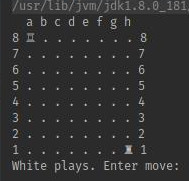
\includegraphics[scale=2.5]{screenshot1}
\end{figure}

Because of the dark theme it appears that the black and white rooks have swapped position from what they should be but I have checked and the correct characters are being printed. When run within a console this will appear correct. \newline

\noindent \textbf{Testing Moving Pieces}

\end{document}